\section{Concept of LEM Simulation Platform}
To start off, this section brings together the previous sections \ref{sec:about_blockchain} and \ref{sec:btm},
and explains how the bundle trading market framework \textit{(BTM)} and a blockchain interact to implement a simulation 
of a local energy market, which are introduced in section \ref{sec:lem}.
Finally, this section gives an example for a linear programming problem in terms of energy efficient demand side management of households. 

First, in the presented market mechanism in section \ref{sec:btm}, independent, self-interested agents trading bundled resources
in a double-auction market. 
In case of the developed open-blockchain based LEM simulation, the agents of the \textit{BTM} respresent households. 
These households are trading independently and self-interested bundles of energy resources 
to minimize the monetary expense through optimally scheduling the operation and energy consumption 
of all energy consuming appliances.

Next, blockchain is introduced as the applied ICT of the developed LEM simulation. 
As already mentioned earlier, the implementation of LEM needs 
local distributed control and management techniques, which can addressed by the blockchain technology.
This implies that the respective households submit and receive all relevant data, informations and payments via a blockchain. 
Moreover, the double-auction market which enables households to trade their energy bundles, is operated by a dealer.
In turn, the dealer is implemented by a smart contract, which are introduced in section \ref{sec:smart_contract}, and a conventional software client. 
The dealers' smart contract contains all relevant information regarding the market mechanism, like submitted orders, trades, 
dealers' inventory and market prices. 
Therefore, the households exclusively communicate with the dealers' smart contract. 

\begin{figure}[htbp]
	\centering
	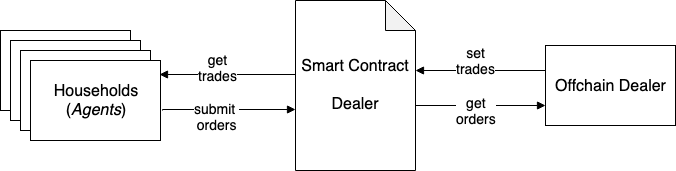
\includegraphics[width=.7\linewidth]{./figures/concept_lem.png}
	\caption{Simplified presentation of the applied communication}
	\label{figure:concept_lem}
\end{figure}

With reference to figure \ref{figure:concept_lem}, the households submit their orders to the dealers' smart contract.  
Afterwards, the dealers' conventional software client, designated as \textit{off-chain} dealer in the figure, fetches all existing orders contained in the smart contract
and solves the \textit{market matching problem}, which is introduced in section \ref{sec:market_clearing_mechanism}.
Secondly, the \textit{off-chain} dealer updates all relevant information in the smart contract, for instance 
the settled orders, the trades, the new market prices and the inventory.
Finally, the households get their respective trades from the dealers' smart contract. 

Anyway, the \textit{off-chain dealer} is necessary due to the complex and costly calculation of the \textit{market matching problem}. 
As mentioned in section \ref{sec:transaction}, each transaction consume gas. Additionally, each mathematical operation in a smart contract
increases the amount of gas to be paid for the respective transaction. As a consequence, implementation and execution of the \textit{market matching problem}
in the smart contract itself would be hard to realize and associated with high transaction costs. 

Hence, a well designed smart contract should move computational complexity \textit{off-chain} 
and focus more on updating state in the contract \shortcite{calculate_cost_eth}. A balance between \textit{on-chain}
and \textit{off-chain} complexity should be found.

In addition, we mentioned in section \ref{sec:btm} that the developed open blockchain-based LEM platform applied a synchronous
call market. That means, the dealer only executes the \textit{market matching problem} after all agents have submitted their orders.
Likewise, we mentioned in section \ref{sec:smart_contract} that smart contracts are only active and run if they called by a transaction.
They will never run on his own or in the background. For this reason, a mechanism is necessary which triggers the execution of the 
\textit{market matching problem}. The implementation of an \textit{off-chain} dealer is also suitable for this.

So far, this section presented the basic idea and concept of the developed open blockchain-based LEM platform
and explained the necessity of all exisiting components. In the following section [ref einfügen!], the setup 
and technical implementation of the simulation will be described in detail. 

However, we stated earlier in this section that the agents of the \textit{BTM} respresent households
and that these households trading bundles of energy resources to minimize the monetary expense. 
In section \ref{sec:btm_problem_overview}, we introduced the individual linear progams of the agents.
Further, we explained in section \ref{sec:agent_bidding} that a rational agent will choose an improving bundle for 
trading which leaves his wealth level on the same level or better off and defined the selection of such a bundle 
as the \textit{bundle determination problem}.
Finally, to embed the \textit{BTM} into the topic of local energy markets, we need to define 
a linear programming problem which depicts the energy efficient demand side management of households.

\subsection{Demand side management of a household}
This subsection will embed the \text{BTM} into the topic of local energy markets. 
Therefore, we will develop a linear programming problem in terms of energy efficient demand side management of households.  
That means, the objective of the respective households is to minimize their monetary expense regarding energy consumption.
However, the minimization of the costs due to energy consuming depends on a number of constraints. 


\begin{comment}

# CONTENT

an agents bundle selection 
can be defined as the following \textit{bundle determination problem:}

rational agent will choose an improving bundle for trading, 
which leaves his wealth level on the same level or better off. 



\end{comment}